% !TeX spellcheck = en_US
\documentclass[a4paper]{report}
\usepackage[T1]{fontenc}
\usepackage[utf8]{inputenc}
\usepackage[english]{babel}
\usepackage{geometry}
\usepackage{graphicx}
\usepackage{subfig}
\usepackage{lipsum}
\usepackage{verbatim}
\usepackage[table,xcdraw]{xcolor}
\geometry{a4paper,top=2.5cm,bottom=2.5cm,left=3cm,right=3cm,%
	heightrounded,bindingoffset=5mm}

\usepackage{color}
\usepackage{listings}
\usepackage{xcolor}
\usepackage{hyperref}

\colorlet{punct}{red!60!black}
\definecolor{background}{HTML}{EEEEEE}
\definecolor{delim}{RGB}{20,105,176}
\colorlet{numb}{magenta!60!black}




\newcommand{\HRule}{\rule{\linewidth}{0.5mm}}

\begin{document}
	\begin{titlepage}
		\begin{center}
			
			% Top 
			
\includegraphics[width=0.45\textwidth]{img/unipi.png}~\\[2.5cm]
			
			
			% Title
			\HRule \\[0.4cm]
			{ \LARGE 
				\Huge\textbf{Intelligent Systems Project Report}\\[0.5cm]
				\LARGE\textit{Author:} \\[0.1cm]
				Francesco Iemma \\[0.1cm]
				%\emph{Francesco Iemma}\\[0.4cm]
			}
			\HRule \\[1.5cm]
			
			
			
			% Author
			{ \Large
			%	\textit{Author:} \\[0.1cm]
			%	Francesco Iemma \\[0.1cm]
			}
			
			\vfill
			
			\textsc{\large M.Sc. in Computer Engineering}\\[0.4cm]
			
			
			% Bottom
			{\large Academic Year 2020/21}
			
		\end{center}
	\end{titlepage}
	
	
	\tableofcontents
	
	\chapter*{Introduction}
	The tasks performed in this project are the following:
	\begin{itemize}
		\item \textit{3.1} "Design and develop two MLP artificial neural networks that accurately estimate a person's valence and arousal, respectively" and "two RBF networks that do the same thing as the MPLPs"
		
		\item \textit{3.3} "Design and develop a fuzzy inference system to fix the deficiencies in the arousal dimension"
		
		\item \textit{4.1} "Design and develop a convolutional neural network (CNN) that accurately classifies a person's emotion, based on facial expression."
	\end{itemize}

	\noindent The dataset at our disposal are two, one for tasks \textit{3.1} and \textit{3.3} and another one for task \textit{4.1}.
	\noindent For what concern the first dataset, i.e. the one with biomedical signals for estimate arousal and valence, it is important to perform a cleaning of the data in order to obtain better performance for the neural networks that will be trained on it. This process, which is performed by the script \texttt{/matlab/data.m} is explained in the \autoref{chap: dataCleaning}. 
	
	\noindent After this chapter for each task is dedicated a chapter in which are explained the choices done and the results obtained in terms of performance.
	
\chapter{Data Cleaning}
	\label{chap: dataCleaning}
	\noindent In this chapter we will see the data cleaning procedure performed in order to obtain better performance for the NNs. The steps done are:
	\begin{itemize}
		\item Remove non numeric values
		\item Remove outliers
		\item Balance the data among the different values of arousal and valence
		\item Features selection
	\end{itemize}
	\noindent All the procedure is contained in the file \texttt{/matlab/data.m}. The first two steps are performed thanks two matlab functions:
	\begin{itemize}
		\item \texttt{isinf(A)} that given a matrix returns a logic matrix is indicated if the correspondent element of the input matrix are infinite ($1$) or not ($0$) 
		
		\item \texttt{rmoutliers(dataset, method)} that given a dataset remove the outliers found using the method specified in input that is 'median' by default (i.e. "Outliers are defined as elements more than three scaled MAD from the median. The scaled MAD is defined as $c\times median(abs(A-median(A))$")
	\end{itemize} 
	
	\noindent Then after the first two steps there are the most interesting part: data balancing and features selection.
	
	\newpage
	\section{Data Balancing}
	\noindent The dataset is composed by samples and each sample contains biomedical signals: to each set of biomedical signals (that we will call \textit{features}) correspond a value for arousal and a value for valence. The possible values are 7 ($1,\; 2.\bar3,\; 3.\bar6,\; 5,\; 6.\bar3,\; 7.\bar6,\; 9$), thus we can divide the dataset according 7 class for arousal and valence. The distribution of the samples among the classes is represented in the histograms in figure \ref{beforeBalancingArousal} and \ref{beforeBalancingValence}.
	
	\begin{figure}[htpb]
		\centering
		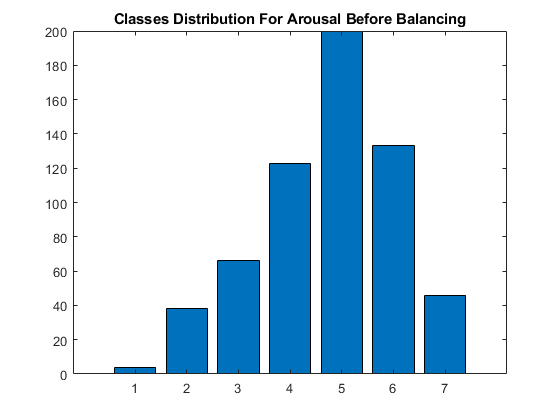
\includegraphics[scale=0.7]{img/beforeBalancingArousal.png}
		\caption{Classes Distribution For Arousal Before Balancing}
		\label{beforeBalancingArousal}
	\end{figure}  

	\begin{figure}[htpb]
		\centering
		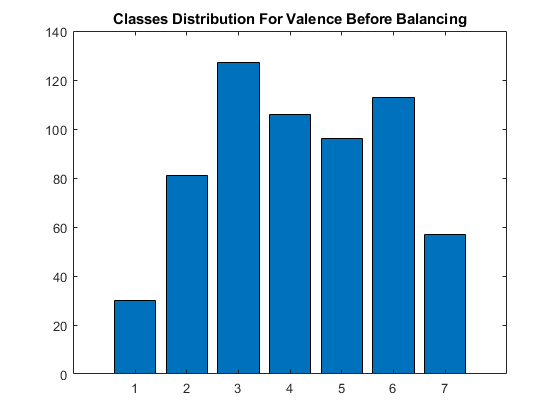
\includegraphics[scale=0.7]{img/beforeBalancingValence.png}
		\caption{Classes Distribution For Valence Before Balancing}
		\label{beforeBalancingValence}
	\end{figure}


\noindent As we can see the samples are heavily unbalanced, for this reason an algorithm to balance the data has been used. The algorithm is based on the concepts of undersampling, oversampling and data augmentation.

\noindent The steps are the following:
\begin{enumerate}
	\item I augment the samples that belong to the majority class of arousal 
	 and don't belong to the majority class of valence and viceversa (i.e. the samples that 
	 belong to the majority class of valence and don't belong to the minority
	 class of arousal).
	 
	 \item I remove the samples that belong to the majority class of 
	 arousal and don't belong to the minority class of valence and viceversa (i.e. the
	 samples that belong to the majority class of valence and don't belong to
	 the minority class of arousal).
	
	 \item I repeat steps 1 and 2 for a $n=40$ ($40$ after some experiments this is the number that gives the best results) times and for each repetition I compute the new majority and minority class both for arousal and valence.
	 
	 \item After the end of the repetitions I perform an undersampling on the first class because it is unbalanced for what concern the valence. Thus I remove some samples from this class, after some experiments removing $30$ samples results in a balanced distribution for both arousal and valence.
\end{enumerate}

\noindent At the end of this procedure the data are balanced as we can see in figure \ref{afterBalancingArousal} and \ref{afterBalancingValence}.

	\begin{figure}[htbp]
		\centering
		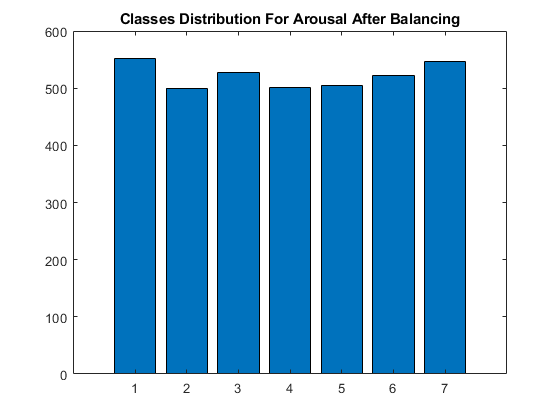
\includegraphics[scale=0.7]{img/afterBalancingArousal.png}
		\caption{Classes Distribution For Arousal After Balancing}
		\label{afterBalancingArousal}
	\end{figure}  
	
		\begin{figure}[htbp]
		\centering
		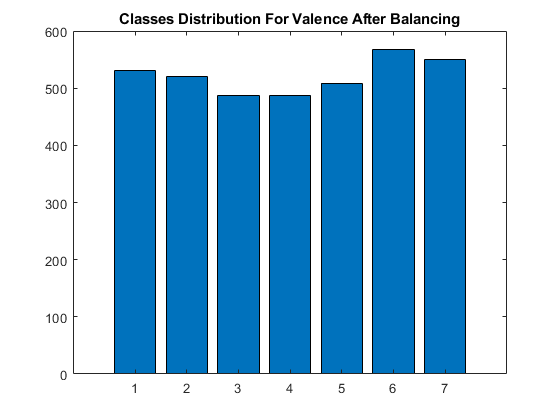
\includegraphics[scale=0.7]{img/afterBalancingValence.png}
		\caption{Classes Distribution For Valence After Balancing}
		\label{afterBalancingValence}
	\end{figure}
	
	\section{Features Selection}
	\noindent Before the features selection is necessary to divide the data in two set: one for training and one for test. This is very important because if we use all the data to perform feature selection we have a bias because the test data have been already seen by the net.
	
	\noindent Thus after the extraction of the holdout partition we perform x CAMBIARE times \texttt{sequentialfs} for arousal and x time for valence. Then we select the first \texttt{FEATURES\_TO\_SELECT} (constant set at the beginning of the script) features that appear most times in the different runs of sequentialfs, this operation is performed separately for arousal and valence.
	
	\noindent At the end we save the data obtained into three \texttt{.mat} files:
	\begin{itemize}
		\item \texttt{/matlab/data/biomedical\_signals/dataset\_cleaned.mat}
		
		\noindent It contains the entire dataset without infinite values, outliers and with balanced class distribution.
		\item \texttt{/matlab/data/biomedical\_signals/training\_data.mat}
		
		\noindent It contains a \texttt{struct} with the training input (only the selected features) and the correspondent target output.
		
		\item \texttt{/matlab/data/biomedical\_signals/test\_data.mat}
		
		\noindent It contains a \texttt{struct} with the test input (only the selected features) and the correspondent expected output.
	\end{itemize}
	
\chapter{Neural Networks}
	\noindent In this chapter we will see two types of neural networks that resolve the same problem, that is to estimate the values of arousal and valence given a set of biomedical signals.	
	\section{Fitnet}
	\section{RBF}
	
	\chapter{Fuzzy Inference System}
	
	\chapter{Convolutional Neural Networks}
\end{document}